\section[Wiring como Hardware]{Wiring como Hardware}

Wiring é pequena placa com microcontrolador e portas "input/output" que são capazes de interagir com componentes externos (sensores, leds, displays) para assim criar sistemas das mais diversas situações de acordo necessidades especificas.

\subsection[Portas de Comunicação]{Portas de Comunicação}

Essas portas "input/output" são compostas por um conjunto de pinos. O tipo de cada pino pode ser definido pelo usuário ou programador para responder as mais diversas situações do mundo físico. Há dois tipos de sinais presentes na placa, o DIGITAL definido por sinal alto e baixo, sendo; ON ou OFF e HIGH ou LOW, e o sinal ANALÓGICO definido por qualquer faixa continua.

A placa tem uma porta USB que pode ser ligada ao seu PC. O programador pode desenvolver códigos através da IDE proprietária e carregá-lo na placa através dessa conexão.
p
\subsection[Estrututa Atual]{Estrututa Atual}

Pela estrutura atual a placa foi projetada para receber prototipagem de 3 formas, sendo:
    \begin{alineas}
        \item Funções interativas e autônomas, sendo o programa carregado na placa sem que ela precise esta conectada ao PC para desenvolvê-las.
	    \item Funções interativas conectadas a um PC que recebem e enviam comandos para um determinada função.
        \item Funções interativas conectadas a uma LAN interligada com dispositivos de hardwares.
    \end{alineas}
	
\subsection[Modelos de Placas]{Modelos de Placas}

Os modelos de placa Wiring disponíveis são: Wiring Mini V1.0 Até Rev. 0004, Wiring Mini com controlador atmega128, Wiring V1.1 Sparkfun com controlador atmega1281, Wiring V1.1 Sparkfun com controlador atmega2561, Wiring S com controlador atmega644p

\subsection[Modelos de Placas]{Modelos de Placas}
Modelos distribuídos por roguerobotics: Wiring M, Wiring XS, Wiring L

\subsection[Detalhe das Portas de Comunicação]{Detalhe das Portas de Comunicação}

Pinagem Input/Output; Digital, Analógico, PWM analógico, Serial, Funções Especiais, Interrupção, LED na placa, Fonte de alimentação.

Resumo da Placa Wiring S com controlador atmega644p (ultima geração)
	- 32 Pinos I/O
	- 8 Entradas Analógicas
	- 2 Portas Seriais
	- 6 PWM com saídas analógicas 
	- SPI
	- TWI
	- 3 pinos de interrupção
    - Regulador de potencia de 3,3V para 5V.

\subsection[Características Portas Digitais]{Características Portas Digitais}

As portas digitais podem serem ligadas de forma individual. E quando ligadas são capazes de receber e enviar sinais ALTOS e BAIXOS semelhantes aos controladores de um determinado aparelho eletrônico podendo executar tal função e consequentemente fazer o ligando o desligamento de diversos modelos de dispositivo (Motores, Lampadas, Eletrodomésticos, etc...)

Todas as placas Wiring possuem dispositivo de alerta visual podendo ser usado para testes de diagnóstico. O Dispositivo é acoplado diretamente a placa mãe chamado de Wled.

\subsection[Características Portas Analógicas]{Características Portas Analógicas}

As portas analógicas comportam tensão de 0-5V. As tensões são revertidas em sinais de números  0 a 1023. 
As entradas podem serem usadas para medir "quantidades continuas". Exemplo: Intensidade de Luz, Temperatura, Sensores analógicos, entre outros.....

\subsection[Portas PWM - Pulse Width Modulation]{Portas PWM - Pulse Width Modulation}

Elas comutam Ligado e Desligado muitas vezes seguidas por milissegundos e simulam comportamento analógico dessa forma é criado efeito baixa ou escurecimento intensidade de luz ou controle da velocidade de um motor. Estas funcionalidades estão disponíveis em pinos específicos.

Placas Wiring V1.x os pinos são: 29, 30, 31, 35, 36 e 37.
Placas Wiring S, os pinos são: 4, 5, 6, 7, 19 e 20.

\subsection[Portas Seriais]{Portas Seriais}

As placas Wiring tem disponível duas portas seriais, são chamadas de "serial" e "serial1".  Sendo elas disponibilizadas através do conector USB e são usadas para interação com dispositivos com esse tipo de comunicação.

Placas Wiring V1.x os pinos são: Serial = 32:rx0 e 33:tx0  Serial1 = 2:rx1 e 3:tx1
Placas Wiring S os pinos são: Serial = 0:rx0 e 1:tx1 Serial1 = 2:tx2 e 3:tx3   

\subsection[Características ISP e TWI - Interface dois Fios i2c]{Características ISP e TWI - Interface dois Fios i2c}

É possível conectar até 128 sensores e ou, atuadores i2c usando apenas duas conexões (2 fios) para fazer essa comunicação. Também há a possibilidade de criar uma rede de até 127 Placas Wiring usando biblioteca especifica Wire. Há dois protocolos sendo; ISP e TWI que respectivamente são tratados pelas bibliotecas SPI e Wire.

Placas Wiring V1.x os pinos ISP: 24(SS), 25(MOSI) 26(MISO) e 27(SCK)  e os TWI: 0(SCL) e 1(SDA) 
Placas Wiring S s pinos do ISP são: 20 (SS), 21 (MOSI), 22 (MISO) e 23 (SCK) e os TWI são: 8 (SCL) e 9 (SDA)

\subsection[Interrupções]{Interrupções}

É possível gerar e atender interrupções externas no hardware da fiação. Existem pinos no hardware da fiação capazes de gerar interrupções externas.

Placas Wiring V1.x os pinos de interrupção são: 0, 1, 2, 3, 36, 37, 38 e 39, nomeados como EI0..EI7.
Placas Wiring S os pinos de interrupção são: 2, 3 e 18, nomeados como EI0, E1 e EI2.

\subsection[Detalhes]{Detalhes}

Nos pinos de hardware da fiação são agrupados em portas. Na maioria dos casos, uma porta é um conjunto de 8 pinos e pode ser usada para enviar ou receber dados para dispositivos em paralelo (8 bits por vez). Eles são úteis ao usar dispositivos como telas de cristal líquido ou impressoras. Cada porta pode ser configurada e usada individualmente como INPUT ou OUTPUT a partir da API do Wiring Framework no ambiente de programação de Fiação através dos comandos portMode, portRead e portWrite.

É possível usar a seção de entrada analógica como uma digital, nesse caso, pinos individuais e a porta continuarão a ser numerados continuamente.
Top LEDs on-board.

O hardware da fiação tem quatro LEDs na placa: um LED de energia mostrando se a placa está ligada, um LED conectado diretamente a um pino digital que pode ser ligado ou desligado.

\subsection[Imagem placa Wiring]{Imagem placa Wiring}
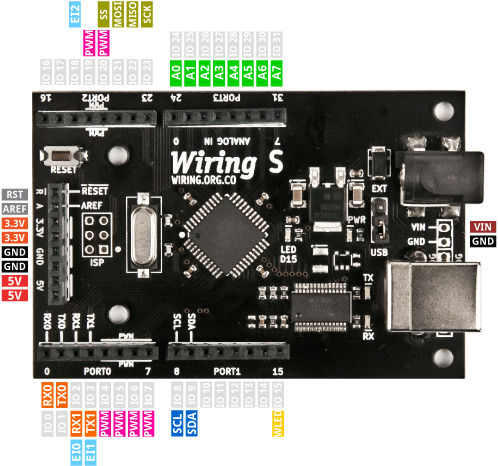
\includegraphics[scale=0.5]{artigo/refs/PinsWiringS.png}


\subsection[Origem]{Origem}
Todas as informações foram extraídas através do site \footnote{\url http://wiring.org.co/hardware/}.

%http://wiring.org.co/hardware/